\chapter{Capsule Network Architectures}\label{chapter:capsules}
A capsule is conceived as a group of neurons whose outputs encode different properties of an entity such as an object or part of an object in an image. The properties could represent instantiation parameters on the object's appearance manifold such as the precise pose, lighting and deformation or the probability that the entity is present. Layers within a capsule network consist of several capsules. Routing between the layers is determined by the votes from the capsules in the lower layer. Capsules can make a guess as to what they expect the higher layer's capsules instantiation parameters to be and cast a vote. Votes are calculated by applying discriminatively learned transformations to the capsules' outputs. The routing algorithm will then determine, based on the lower capsules' votes, which higher layer capsules to activate. The goal of capsule networks is to achieve invariance regarding their capsules' instantiation parameters. A specific capsule architecture is largely defined by the nature of its routing algorithm and the dimension of its output as well as the order of the tensors used to compute the votes.

\section{Transforming Auto-encoders}
The first publication on capsules came from Hinton et al. in the form of transforming auto-encoders in 2011 \cite{hinton2011transforming}. These capsules encoded the instantiation parameters of their internal representation together with the probability that the learned entity is present into a small output vector. Each capsule would learn to recognize a single visual entity over a limited subdomain of its appearance manifold. Ideally, the probability would be locally invariant as long as the instantiation parameters remain within the trained submanifold. This is in contrast to the instantiation parameters, which are equivariant. Meaning as the viewing conditions change, the parameters encoding the appearance change by an equal amount.

The transforming auto-encoders introduced by Hinton et al. in 2011 were already motivated by a desire to retain precise part-whole relationships, which are lost by the pooling operations in convolutional neural networks (cf. section \ref{section:limitations}). If a capsule can be trained to encode the pose of the visual entity it represents in its output vector, it is a simple matter to test whether two capsules $A$ and $B$ are in agreement about a higher level capsule $C$. To see this, suppose that the matrix $\vb{T}_{A/B}$ is the pose between the canonical entity as learned by the capsule $A$ or $B$ respectively and the current instantiation. Multiplying this with the part-whole transformation matrix $\vb{T}_{A/B\rightarrow C}$ will result in a prediction for the pose of capsule $C$'s entity. Now, if
\begin{align}
    \vb{T}_A\vb{T}_{A\rightarrow C} \approx \vb{T}_B\vb{T}_{B\rightarrow C},
\end{align}
then the capsules are a close match and activate capsule $C$. Hinton et al. argue that this naturally leads to precise part-whole relationships. If the entities of capsules $A$ and $B$ e.g. correspond to a mouth and a nose respectively, then they have to be in right spatial relationship to form a face if they activate the higher capsule $C$ representing the whole face. The pose of capsule $C$ can then be determined by the average of the lower capsules' votes.
\begin{align}
    \vb{T_C} = \sum_{i\in \{A, B\}} \vb{T}_i\vb{T}_{i\rightarrow C}
\end{align}
This means that except for the first layer of capsules, only the viewpoint invariant part-whole transformations have to be learned, while the entity poses are encoded in the neural activities at run time. The rest of the paper focuses on how to extract the poses from the pixel intensities for the first layer. This was done by training capsules on transformed image pairs and providing the capsules with non-visual access to the transformation. Hinton et al. justified this by pointing out that the human visual system is also provided with information about the eye-movement while saccades correspond to a translational transformation of the retinal image.
\begin{figure}
    \centering
    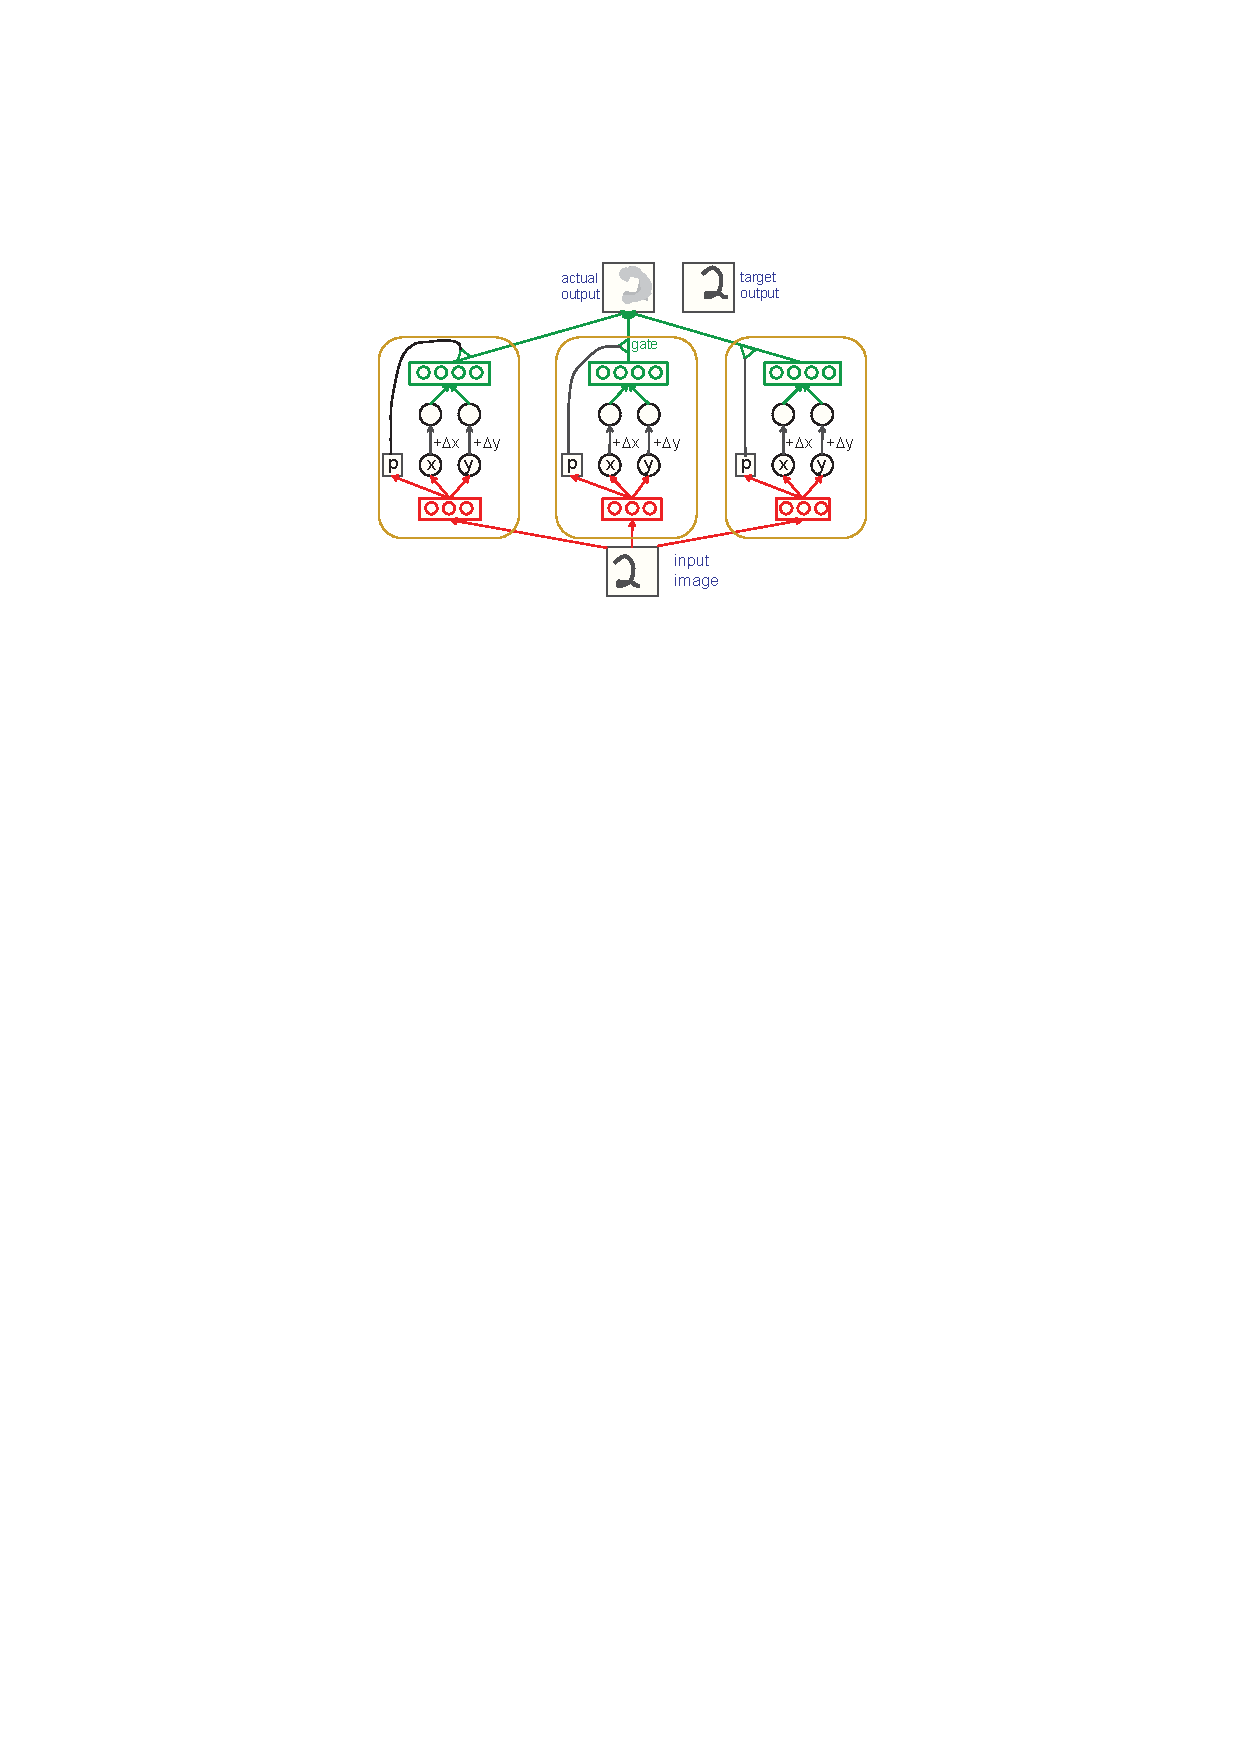
\includegraphics[width=.75\textwidth]{figures/caps-fig1.pdf}
\caption[Capsules in a transforming auto-encoders]{Capsules in a transforming auto-encoder. The network consists of a single layer of capsules. Each capsule includes hidden recognition (in red) and generation units (in green). During training transformation parameters (in this case the translations $\Delta x$ and $\Delta y$) as well as the transformed image are provided to the network. A capsule's output vector is further multiplied with its probability, thus muting capsules with a low probability.}\label{fig:auto-encoders}
\end{figure}\noindent

These first capsule networks actually consisted of only one layer of capsules and did not include the routing mechanism of later implementations. Instead, they included two internal layers of logistic neurons, termed recognition and generation units respectively (cf. figure \ref{fig:auto-encoders}). The recognition units were trained to extract pose parameters and the probability that the visual entity is present directly from the provided image. A capsule's input could be constrained to a fixed receptive field with the capsules aligned in a grid across the image. The capsules then apply a transformation to the pose and provide the generation units with this information. The generation units on the other hand were trained to output the transformed part of the input image centered at the capsule's receptive field. All the neurons within a capsule were trained discriminatively using gradient descent with backpropagation. The training signal was provided by a form of reconstruction loss where the capsules had access to the transformation and the input and reconstruction target were the original and transformed images respectively. The transforming auto-encoders were able to learn poses in the form of $3x3$ matrices and could be used to successfully apply affine transformations. However, they were limited to one layer of capsules and could not be scaled effectively, as the capsules were fixed to a single position. Also they were only able to learn properties, that could be controlled and provided in explicit non-visual form to the network.
\section{Dynamic Routing Between Capsules}
\section{Matrix Capsules With EM Routing}